%- %%%%

\chapter{Stato dell'arte}
\label{chap:art}

%%%%

\section{Introduzione}
\label{chap:art-intro}
Con l'avvento delle tecnologie per il sequenziamento del DNA partendo da singole cellule (SCS), iniziano ad essere disponibili dati di alta qualità. Queste tecnologie forniscono il sequenziamento di dati da singole cellule, permettendo quindi di ricostruire l'albero filogenetico di una cellula. È però da tenere in considerazione l'alto tasso di errore associato a questo tipo di dati, innalzando di conseguenza il grado di difficoltà del processo di ricostruzione della filogenesi. 
In questo capitolo, verranno esaminate le tecnologie già presenti che hanno affrontato questa sfida, focalizzando l'analisi sul modello di ricerca dell'ottimo, del calcolo della \textit{likelihood} dell'albero inferito e della complessità dell'algoritmo utilizzato.

%%%%

\section{SciTe \cite{scite}}
\label{chap:art-scite}
SCITE (\textit{Single-Cell Inference of Tumor Evolution}) usa un approccio basato sulla likelihood dell'albero inferito per fare una ricerca stocastica dell'albero migliore rispetto ai dati in input. Ricordando l'assunzione che le mutazioni siano indipendenti l'una dall'altra, dati i tassi di errore $\theta = (\alpha, \beta)$, la matrice $M$ di partenza di dimensioni $n \times m$, dove $n$ è il numero di cellule e $m$ il numero di mutazioni, possiamo calcolare la likelihood come segue:
\begin{equation}
  P(M | T, \sigma, \theta) = \prod_{i = 1}^{n}\prod_{j = 1}^{m} P(M_{i,j} | D_{i,j})
\end{equation}
Lo strumento è costruito attorno al funzionamento di una catena di Markov Monte Carlo (\autoref{chap:intro-extra-markov-mc}) che permette di trovare l'albero migliore basandosi sulla likelihood calcolata, oppure basandosi sulla distribuzione a posteriori. Uno dei principali vantaggi indicati è quello della scalabilità lineare, proporzionale con il numero dei campioni.

\subsection{Complessità}
Ad ogni step, la MCMC impiega $O(mn)$ per calcolare la likelihood dell'albero, impiegando un tempos stimato di $O(mn^3 ln(n))$ per una convergenza all'albero migliore. Il tempo è linearmente dipendente con il numero dei campioni e di mutazioni.

\section{SiFit: inferring tumor trees from single-cell sequencing data under finite-sites models \cite{sifit}}
\label{chap:art-sifit}
Il progetto \textit{SiFit} affronta il problema presupponendo un modello a posizioni finite (\textit{finite sites model}), quindi permettendo delle back-mutation\footnote{Mutazioni all'indietro, una mutazione viene persa durante la vita di una cellula}.
Lo strumento accetta sia matrici binarie, con un set di valori possibili $\{ 0, 1, X \}$, che matrici ternarie, per le quali accetta il set di valori $\{ 0, 1, 2, X \}$, dove $0$ denota un genotipo \textit{reference} omozigota, $1$ e $2$ denotano un genotipo eterozigota ed omozigota \textit{non-reference}, rispettivamente, e $X$ denota la mancanza di informazioni.

Vengono principalmente usati due tipi di mosse: mosse di \textit{prune and regraft} e mosse di \textit{swap}. Le mosse di \textit{prune and regraft} prevedono il cambiamento randomico della topologia dell'albero attraverso il riposizionamento di un sottoalbero all'interno (rSPR, \textit{random Subtree Prune and Regraft}) e la lunghezza dei rami dell'albero (eSPR, \textit{extending Subtree Pruning and Regrafting}). Le mosse di \textit{swap} prevedono lo scambio di nodi interni all'albero (stNNI, \textit{stochastic nearest-neighbour interchange}) e dei rami (rSTS, \textit{random Sub-Tree Swapping}) \cite{sifit, efficiencymcmc}.

\subsection{Complessità}
Ad ogni passo dell'algoritmo proposto, calcolare la \textit{likelihood} dell'albero è il processo più dispendioso. Per $n$ singole cellule e $m$ mutazioni, il calcolo della likelihood impiega $\mathcal{O} (nk^2m)$, dove $k$ è il numero massimo di stati per mutazione, quindi $k = 3$ e $k = 2$ per una matrice ternaria e una matrice binaria in input, rispettivamente.

Il numero di iterazioni $i$ è definito dall'utente, ottenendo quindi come complessità generale dell'algoritmo $\mathcal{O}(nk^2mi)$.

\section{SASC - Inferring Cancer Progression from Single-Cell Sequencing while Allowing Mutation Losses \cite{SCiccolellaSasc}}
\label{chap:art-sasc}
In SASC (\textit{Simulated Annealing Single-Cell} inference) viene utilizzato il modello \textit{finite-sites} insieme al modello di Dollo-\textit{k}. Il modello della Parsimonia di Dollo prevede che ogni mutazione può essere acquisita una sola volta, ma una perdita di una mutazione può accadere un numero indefinito di volte. La versione ristretta di Dollo-\textit{k} assume che ogni mutazione possa essere acquisita una sola volta e persa al massimo $k$ volte. Per trovare l'albero migliore il problema viene modellato sull'algoritmo euristico \textit{simulated annealing} (\autoref{chap:intro-optim-sa}). Le mosse utili alla scalata della collina sono: \textit{aggiunta di back-mutation}, \textit{rimuzione di back-mutation}, \textit{node switch} e \textit{prune-and-regraft}.

\begin{figure}[h]
  \centering
  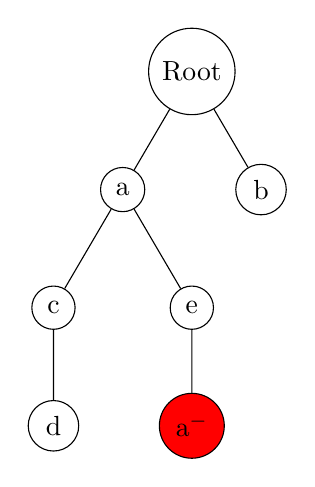
\begin{tikzpicture}[sibling distance=5em,every node/.style = {shape=circle,draw, align=center}]
    \node {Root}
            child { node {a} 
            child { node {c} 
            child { node {d}  } }
            child { node {e} 
            child { node [fill=red] {a$^-$}  } } }
            child { node {b}  };
    \end{tikzpicture}
  \caption{Esempio di back-mutation}
  \label{fig:art-sasc-bm}
\end{figure}

Ad ogni riduzione della temperatura viene cercato un albero topologicamente vicino a quello attuale applicando una delle quattro operazioni precedenti, finché non si raggiunge la temperatura minima. La bontà dell'albero è definita dalla \textit{likelihood logaritmica}, e viene calcolata ad ogni operazione effettuata sull'albero inferito nella seguente maniera:

\begin{equation}
  \label{eq:art-sasc-lh}
  max \sum_i^n \sum_j^m \log ( P( M_{i,j} | D_{i,j} ) )
\end{equation}

\subsection{Complessità}
L'algoritmo Simulated Annealing impiega $O(\log t)$ step fino a quando non raggiunge la temperatura minima, con $t$ ad indicare la temperatura di partenza, e per ogni step impiega $O(n m)$ per calcolare la likelihood logaritmica. In generale, SASC ha una complessità di $O(nm \log t)$.
% TODO: check complexity calculation for SASC

  